% Created by tikzDevice version 0.12.6 on 2025-05-06 22:53:33
% !TEX encoding = UTF-8 Unicode
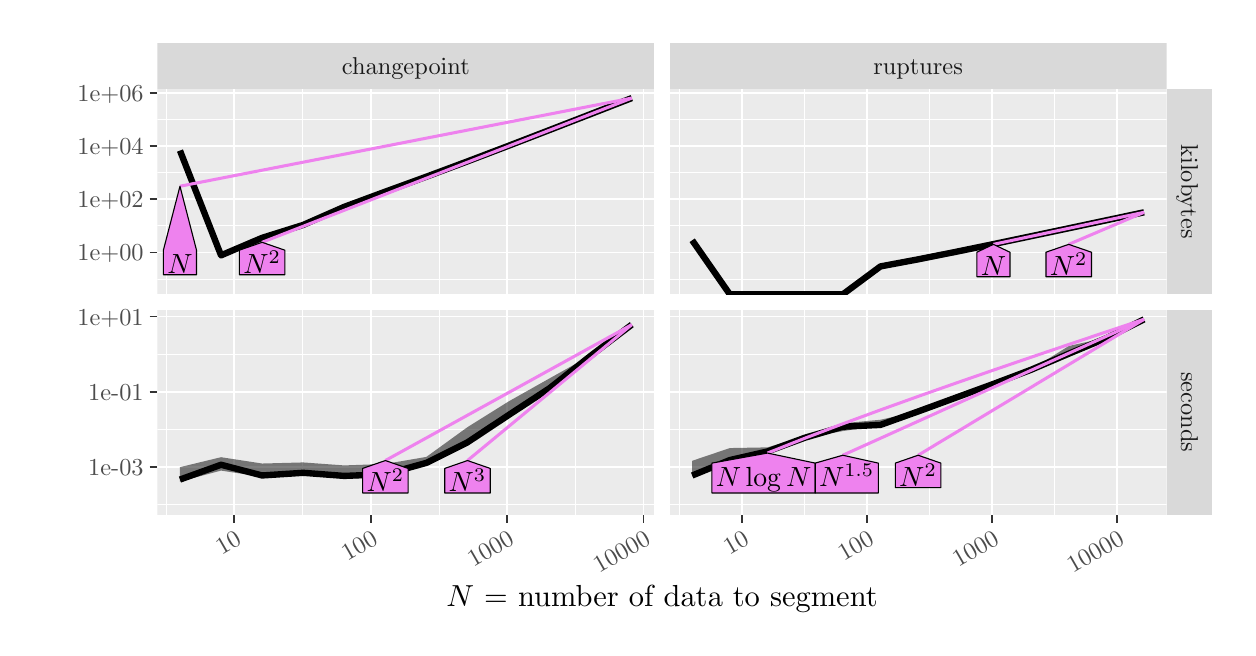
\begin{tikzpicture}[x=1pt,y=1pt]
\definecolor{fillColor}{RGB}{255,255,255}
\path[use as bounding box,fill=fillColor,fill opacity=0.00] (0,0) rectangle (433.62,216.81);
\begin{scope}
\path[clip] (  0.00,  0.00) rectangle (433.62,216.81);
\definecolor{drawColor}{RGB}{255,255,255}
\definecolor{fillColor}{RGB}{255,255,255}

\path[draw=drawColor,line width= 0.6pt,line join=round,line cap=round,fill=fillColor] ( -0.00,  0.00) rectangle (433.62,216.81);
\end{scope}
\begin{scope}
\path[clip] ( 46.86,120.44) rectangle (226.46,194.74);
\definecolor{fillColor}{gray}{0.92}

\path[fill=fillColor] ( 46.86,120.44) rectangle (226.46,194.74);
\definecolor{drawColor}{RGB}{255,255,255}

\path[draw=drawColor,line width= 0.3pt,line join=round] ( 46.86,125.99) --
	(226.46,125.99);

\path[draw=drawColor,line width= 0.3pt,line join=round] ( 46.86,145.23) --
	(226.46,145.23);

\path[draw=drawColor,line width= 0.3pt,line join=round] ( 46.86,164.47) --
	(226.46,164.47);

\path[draw=drawColor,line width= 0.3pt,line join=round] ( 46.86,183.70) --
	(226.46,183.70);

\path[draw=drawColor,line width= 0.3pt,line join=round] ( 50.00,120.44) --
	( 50.00,194.74);

\path[draw=drawColor,line width= 0.3pt,line join=round] ( 99.30,120.44) --
	( 99.30,194.74);

\path[draw=drawColor,line width= 0.3pt,line join=round] (148.61,120.44) --
	(148.61,194.74);

\path[draw=drawColor,line width= 0.3pt,line join=round] (197.91,120.44) --
	(197.91,194.74);

\path[draw=drawColor,line width= 0.6pt,line join=round] ( 46.86,135.61) --
	(226.46,135.61);

\path[draw=drawColor,line width= 0.6pt,line join=round] ( 46.86,154.85) --
	(226.46,154.85);

\path[draw=drawColor,line width= 0.6pt,line join=round] ( 46.86,174.08) --
	(226.46,174.08);

\path[draw=drawColor,line width= 0.6pt,line join=round] ( 46.86,193.32) --
	(226.46,193.32);

\path[draw=drawColor,line width= 0.6pt,line join=round] ( 74.65,120.44) --
	( 74.65,194.74);

\path[draw=drawColor,line width= 0.6pt,line join=round] (123.95,120.44) --
	(123.95,194.74);

\path[draw=drawColor,line width= 0.6pt,line join=round] (173.26,120.44) --
	(173.26,194.74);

\path[draw=drawColor,line width= 0.6pt,line join=round] (222.56,120.44) --
	(222.56,194.74);
\definecolor{drawColor}{RGB}{0,0,0}

\path[draw=drawColor,line width= 2.3pt,line join=round] ( 55.03,172.40) --
	( 69.87,134.54) --
	( 84.71,140.87) --
	( 99.55,145.53) --
	(114.40,152.07) --
	(129.24,157.56) --
	(144.08,162.96) --
	(158.92,168.49) --
	(173.77,174.13) --
	(188.61,179.84) --
	(203.45,185.59) --
	(218.29,191.36);
\definecolor{drawColor}{RGB}{238,130,238}

\path[draw=drawColor,line width= 1.1pt,line join=round] ( 84.71,139.25) --
	( 99.55,145.04) --
	(114.40,150.83) --
	(129.24,156.62) --
	(144.08,162.41) --
	(158.92,168.20) --
	(173.77,173.99) --
	(188.61,179.78) --
	(203.45,185.57) --
	(218.29,191.36);

\path[draw=drawColor,line width= 1.1pt,line join=round] ( 55.03,159.51) --
	( 69.87,162.41) --
	( 84.71,165.30) --
	( 99.55,168.20) --
	(114.40,171.09) --
	(129.24,173.99) --
	(144.08,176.89) --
	(158.92,179.78) --
	(173.77,182.68) --
	(188.61,185.57) --
	(203.45,188.47) --
	(218.29,191.36);
\end{scope}
\begin{scope}
\path[clip] ( 46.86,120.44) rectangle (226.46,194.74);
\definecolor{drawColor}{RGB}{0,0,0}
\definecolor{fillColor}{RGB}{238,130,238}

\path[draw=drawColor,line width= 0.4pt,line join=round,line cap=round,fill=fillColor] ( 76.48,136.40) --
	( 84.71,139.25) --
	( 92.94,136.40) --
	( 92.94,127.54) --
	( 76.48,127.54) --
	cycle;

\path[draw=drawColor,line width= 0.4pt,line join=round,line cap=round,fill=fillColor] ( 49.04,136.40) --
	( 55.03,159.51) --
	( 61.01,136.40) --
	( 61.01,127.54) --
	( 49.04,127.54) --
	cycle;

\node[text=drawColor,anchor=base,inner sep=0pt, outer sep=0pt, scale=  1.00] at ( 84.71,128.09) {$N^2$};

\node[text=drawColor,anchor=base,inner sep=0pt, outer sep=0pt, scale=  1.00] at ( 55.03,128.09) {$N$};
\end{scope}
\begin{scope}
\path[clip] ( 46.86, 40.64) rectangle (226.46,114.94);
\definecolor{fillColor}{gray}{0.92}

\path[fill=fillColor] ( 46.86, 40.64) rectangle (226.46,114.94);
\definecolor{drawColor}{RGB}{255,255,255}

\path[draw=drawColor,line width= 0.3pt,line join=round] ( 46.86, 44.40) --
	(226.46, 44.40);

\path[draw=drawColor,line width= 0.3pt,line join=round] ( 46.86, 71.59) --
	(226.46, 71.59);

\path[draw=drawColor,line width= 0.3pt,line join=round] ( 46.86, 98.78) --
	(226.46, 98.78);

\path[draw=drawColor,line width= 0.3pt,line join=round] ( 50.00, 40.64) --
	( 50.00,114.94);

\path[draw=drawColor,line width= 0.3pt,line join=round] ( 99.30, 40.64) --
	( 99.30,114.94);

\path[draw=drawColor,line width= 0.3pt,line join=round] (148.61, 40.64) --
	(148.61,114.94);

\path[draw=drawColor,line width= 0.3pt,line join=round] (197.91, 40.64) --
	(197.91,114.94);

\path[draw=drawColor,line width= 0.6pt,line join=round] ( 46.86, 58.00) --
	(226.46, 58.00);

\path[draw=drawColor,line width= 0.6pt,line join=round] ( 46.86, 85.19) --
	(226.46, 85.19);

\path[draw=drawColor,line width= 0.6pt,line join=round] ( 46.86,112.38) --
	(226.46,112.38);

\path[draw=drawColor,line width= 0.6pt,line join=round] ( 74.65, 40.64) --
	( 74.65,114.94);

\path[draw=drawColor,line width= 0.6pt,line join=round] (123.95, 40.64) --
	(123.95,114.94);

\path[draw=drawColor,line width= 0.6pt,line join=round] (173.26, 40.64) --
	(173.26,114.94);

\path[draw=drawColor,line width= 0.6pt,line join=round] (222.56, 40.64) --
	(222.56,114.94);
\definecolor{fillColor}{RGB}{0,0,0}

\path[fill=fillColor,fill opacity=0.50] ( 55.03, 58.00) --
	( 69.87, 61.60) --
	( 84.71, 59.31) --
	( 99.55, 59.71) --
	(114.40, 58.63) --
	(129.24, 59.16) --
	(144.08, 61.71) --
	(158.92, 72.45) --
	(173.77, 81.74) --
	(188.61, 90.10) --
	(203.45, 98.38) --
	(218.29,109.54) --
	(218.29,109.46) --
	(203.45, 98.22) --
	(188.61, 86.26) --
	(173.77, 76.01) --
	(158.92, 66.75) --
	(144.08, 59.17) --
	(129.24, 54.26) --
	(114.40, 53.86) --
	( 99.55, 55.64) --
	( 84.71, 54.50) --
	( 69.87, 56.76) --
	( 55.03, 52.79) --
	cycle;

\path[] ( 55.03, 58.00) --
	( 69.87, 61.60) --
	( 84.71, 59.31) --
	( 99.55, 59.71) --
	(114.40, 58.63) --
	(129.24, 59.16) --
	(144.08, 61.71) --
	(158.92, 72.45) --
	(173.77, 81.74) --
	(188.61, 90.10) --
	(203.45, 98.38) --
	(218.29,109.54);

\path[] (218.29,109.46) --
	(203.45, 98.22) --
	(188.61, 86.26) --
	(173.77, 76.01) --
	(158.92, 66.75) --
	(144.08, 59.17) --
	(129.24, 54.26) --
	(114.40, 53.86) --
	( 99.55, 55.64) --
	( 84.71, 54.50) --
	( 69.87, 56.76) --
	( 55.03, 52.79);
\definecolor{drawColor}{RGB}{0,0,0}

\path[draw=drawColor,line width= 2.3pt,line join=round] ( 55.03, 53.52) --
	( 69.87, 58.87) --
	( 84.71, 55.00) --
	( 99.55, 55.96) --
	(114.40, 54.84) --
	(129.24, 55.43) --
	(144.08, 59.55) --
	(158.92, 66.97) --
	(173.77, 76.82) --
	(188.61, 86.54) --
	(203.45, 98.25) --
	(218.29,109.50);
\definecolor{drawColor}{RGB}{238,130,238}

\path[draw=drawColor,line width= 1.1pt,line join=round] (129.24, 60.39) --
	(144.08, 68.57) --
	(158.92, 76.76) --
	(173.77, 84.94) --
	(188.61, 93.13) --
	(203.45,101.31) --
	(218.29,109.50);

\path[draw=drawColor,line width= 1.1pt,line join=round] (158.92, 60.39) --
	(173.77, 72.67) --
	(188.61, 84.94) --
	(203.45, 97.22) --
	(218.29,109.50);
\end{scope}
\begin{scope}
\path[clip] ( 46.86, 40.64) rectangle (226.46,114.94);
\definecolor{drawColor}{RGB}{0,0,0}
\definecolor{fillColor}{RGB}{238,130,238}

\path[draw=drawColor,line width= 0.4pt,line join=round,line cap=round,fill=fillColor] (121.01, 57.54) --
	(129.24, 60.39) --
	(137.47, 57.54) --
	(137.47, 48.68) --
	(121.01, 48.68) --
	cycle;

\path[draw=drawColor,line width= 0.4pt,line join=round,line cap=round,fill=fillColor] (150.70, 57.54) --
	(158.92, 60.39) --
	(167.15, 57.54) --
	(167.15, 48.68) --
	(150.70, 48.68) --
	cycle;

\node[text=drawColor,anchor=base,inner sep=0pt, outer sep=0pt, scale=  1.00] at (129.24, 49.23) {$N^2$};

\node[text=drawColor,anchor=base,inner sep=0pt, outer sep=0pt, scale=  1.00] at (158.92, 49.23) {$N^3$};
\end{scope}
\begin{scope}
\path[clip] (231.96,120.44) rectangle (411.55,194.74);
\definecolor{fillColor}{gray}{0.92}

\path[fill=fillColor] (231.96,120.44) rectangle (411.55,194.74);
\definecolor{drawColor}{RGB}{255,255,255}

\path[draw=drawColor,line width= 0.3pt,line join=round] (231.96,125.99) --
	(411.55,125.99);

\path[draw=drawColor,line width= 0.3pt,line join=round] (231.96,145.23) --
	(411.55,145.23);

\path[draw=drawColor,line width= 0.3pt,line join=round] (231.96,164.47) --
	(411.55,164.47);

\path[draw=drawColor,line width= 0.3pt,line join=round] (231.96,183.70) --
	(411.55,183.70);

\path[draw=drawColor,line width= 0.3pt,line join=round] (235.51,120.44) --
	(235.51,194.74);

\path[draw=drawColor,line width= 0.3pt,line join=round] (280.70,120.44) --
	(280.70,194.74);

\path[draw=drawColor,line width= 0.3pt,line join=round] (325.90,120.44) --
	(325.90,194.74);

\path[draw=drawColor,line width= 0.3pt,line join=round] (371.10,120.44) --
	(371.10,194.74);

\path[draw=drawColor,line width= 0.6pt,line join=round] (231.96,135.61) --
	(411.55,135.61);

\path[draw=drawColor,line width= 0.6pt,line join=round] (231.96,154.85) --
	(411.55,154.85);

\path[draw=drawColor,line width= 0.6pt,line join=round] (231.96,174.08) --
	(411.55,174.08);

\path[draw=drawColor,line width= 0.6pt,line join=round] (231.96,193.32) --
	(411.55,193.32);

\path[draw=drawColor,line width= 0.6pt,line join=round] (258.11,120.44) --
	(258.11,194.74);

\path[draw=drawColor,line width= 0.6pt,line join=round] (303.30,120.44) --
	(303.30,194.74);

\path[draw=drawColor,line width= 0.6pt,line join=round] (348.50,120.44) --
	(348.50,194.74);

\path[draw=drawColor,line width= 0.6pt,line join=round] (393.69,120.44) --
	(393.69,194.74);
\definecolor{drawColor}{RGB}{0,0,0}

\path[draw=drawColor,line width= 2.3pt,line join=round] (240.12,139.98) --
	(253.73,120.44) --
	(267.33,120.44) --
	(280.94,120.44) --
	(294.54,120.44) --
	(308.15,130.54) --
	(321.75,133.09) --
	(335.36,135.80) --
	(348.96,138.60) --
	(362.57,141.45) --
	(376.17,144.32) --
	(389.78,147.21) --
	(403.39,150.09);
\definecolor{drawColor}{RGB}{238,130,238}

\path[draw=drawColor,line width= 1.1pt,line join=round] (376.17,138.51) --
	(389.78,144.30) --
	(403.39,150.09);

\path[draw=drawColor,line width= 1.1pt,line join=round] (348.96,138.51) --
	(362.57,141.41) --
	(376.17,144.30) --
	(389.78,147.20) --
	(403.39,150.09);
\end{scope}
\begin{scope}
\path[clip] (231.96,120.44) rectangle (411.55,194.74);
\definecolor{drawColor}{RGB}{0,0,0}
\definecolor{fillColor}{RGB}{238,130,238}

\path[draw=drawColor,line width= 0.4pt,line join=round,line cap=round,fill=fillColor] (367.95,135.67) --
	(376.17,138.51) --
	(384.40,135.67) --
	(384.40,126.80) --
	(367.95,126.80) --
	cycle;

\path[draw=drawColor,line width= 0.4pt,line join=round,line cap=round,fill=fillColor] (342.98,135.67) --
	(348.96,138.51) --
	(354.95,135.67) --
	(354.95,126.80) --
	(342.98,126.80) --
	cycle;

\node[text=drawColor,anchor=base,inner sep=0pt, outer sep=0pt, scale=  1.00] at (376.17,127.36) {$N^2$};

\node[text=drawColor,anchor=base,inner sep=0pt, outer sep=0pt, scale=  1.00] at (348.96,127.36) {$N$};
\end{scope}
\begin{scope}
\path[clip] (231.96, 40.64) rectangle (411.55,114.94);
\definecolor{fillColor}{gray}{0.92}

\path[fill=fillColor] (231.96, 40.64) rectangle (411.55,114.94);
\definecolor{drawColor}{RGB}{255,255,255}

\path[draw=drawColor,line width= 0.3pt,line join=round] (231.96, 44.40) --
	(411.55, 44.40);

\path[draw=drawColor,line width= 0.3pt,line join=round] (231.96, 71.59) --
	(411.55, 71.59);

\path[draw=drawColor,line width= 0.3pt,line join=round] (231.96, 98.78) --
	(411.55, 98.78);

\path[draw=drawColor,line width= 0.3pt,line join=round] (235.51, 40.64) --
	(235.51,114.94);

\path[draw=drawColor,line width= 0.3pt,line join=round] (280.70, 40.64) --
	(280.70,114.94);

\path[draw=drawColor,line width= 0.3pt,line join=round] (325.90, 40.64) --
	(325.90,114.94);

\path[draw=drawColor,line width= 0.3pt,line join=round] (371.10, 40.64) --
	(371.10,114.94);

\path[draw=drawColor,line width= 0.6pt,line join=round] (231.96, 58.00) --
	(411.55, 58.00);

\path[draw=drawColor,line width= 0.6pt,line join=round] (231.96, 85.19) --
	(411.55, 85.19);

\path[draw=drawColor,line width= 0.6pt,line join=round] (231.96,112.38) --
	(411.55,112.38);

\path[draw=drawColor,line width= 0.6pt,line join=round] (258.11, 40.64) --
	(258.11,114.94);

\path[draw=drawColor,line width= 0.6pt,line join=round] (303.30, 40.64) --
	(303.30,114.94);

\path[draw=drawColor,line width= 0.6pt,line join=round] (348.50, 40.64) --
	(348.50,114.94);

\path[draw=drawColor,line width= 0.6pt,line join=round] (393.69, 40.64) --
	(393.69,114.94);
\definecolor{fillColor}{RGB}{0,0,0}

\path[fill=fillColor,fill opacity=0.50] (240.12, 60.30) --
	(253.73, 64.90) --
	(267.33, 65.15) --
	(280.94, 69.28) --
	(294.54, 73.86) --
	(308.15, 75.13) --
	(321.75, 78.18) --
	(335.36, 83.17) --
	(348.96, 88.17) --
	(362.57, 93.25) --
	(376.17,101.77) --
	(389.78,104.80) --
	(403.39,111.56) --
	(403.39,111.28) --
	(389.78,104.61) --
	(376.17, 98.60) --
	(362.57, 93.17) --
	(348.96, 88.03) --
	(335.36, 83.04) --
	(321.75, 78.08) --
	(308.15, 73.15) --
	(294.54, 71.03) --
	(280.94, 68.63) --
	(267.33, 63.57) --
	(253.73, 60.00) --
	(240.12, 54.65) --
	cycle;

\path[] (240.12, 60.30) --
	(253.73, 64.90) --
	(267.33, 65.15) --
	(280.94, 69.28) --
	(294.54, 73.86) --
	(308.15, 75.13) --
	(321.75, 78.18) --
	(335.36, 83.17) --
	(348.96, 88.17) --
	(362.57, 93.25) --
	(376.17,101.77) --
	(389.78,104.80) --
	(403.39,111.56);

\path[] (403.39,111.28) --
	(389.78,104.61) --
	(376.17, 98.60) --
	(362.57, 93.17) --
	(348.96, 88.03) --
	(335.36, 83.04) --
	(321.75, 78.08) --
	(308.15, 73.15) --
	(294.54, 71.03) --
	(280.94, 68.63) --
	(267.33, 63.57) --
	(253.73, 60.00) --
	(240.12, 54.65);
\definecolor{drawColor}{RGB}{0,0,0}

\path[draw=drawColor,line width= 2.3pt,line join=round] (240.12, 54.98) --
	(253.73, 60.57) --
	(267.33, 63.67) --
	(280.94, 68.67) --
	(294.54, 72.61) --
	(308.15, 73.27) --
	(321.75, 78.12) --
	(335.36, 83.10) --
	(348.96, 88.07) --
	(362.57, 93.19) --
	(376.17, 98.98) --
	(389.78,104.62) --
	(403.39,111.42);
\definecolor{drawColor}{RGB}{238,130,238}

\path[draw=drawColor,line width= 1.1pt,line join=round] (267.33, 63.09) --
	(280.94, 68.50) --
	(294.54, 73.67) --
	(308.15, 78.68) --
	(321.75, 83.56) --
	(335.36, 88.35) --
	(348.96, 93.06) --
	(362.57, 97.72) --
	(376.17,102.32) --
	(389.78,106.89) --
	(403.39,111.42);

\path[draw=drawColor,line width= 1.1pt,line join=round] (294.54, 62.31) --
	(308.15, 68.44) --
	(321.75, 74.58) --
	(335.36, 80.72) --
	(348.96, 86.86) --
	(362.57, 93.00) --
	(376.17, 99.14) --
	(389.78,105.28) --
	(403.39,111.42);

\path[draw=drawColor,line width= 1.1pt,line join=round] (321.75, 62.31) --
	(335.36, 70.49) --
	(348.96, 78.68) --
	(362.57, 86.86) --
	(376.17, 95.05) --
	(389.78,103.23) --
	(403.39,111.42);
\end{scope}
\begin{scope}
\path[clip] (231.96, 40.64) rectangle (411.55,114.94);
\definecolor{drawColor}{RGB}{0,0,0}
\definecolor{fillColor}{RGB}{238,130,238}

\path[draw=drawColor,line width= 0.4pt,line join=round,line cap=round,fill=fillColor] (247.22, 59.46) --
	(267.33, 63.09) --
	(284.57, 59.46) --
	(284.57, 48.65) --
	(247.22, 48.65) --
	cycle;

\path[draw=drawColor,line width= 0.4pt,line join=round,line cap=round,fill=fillColor] (284.57, 59.46) --
	(294.54, 62.31) --
	(307.39, 59.46) --
	(307.39, 48.65) --
	(284.57, 48.65) --
	cycle;

\path[draw=drawColor,line width= 0.4pt,line join=round,line cap=round,fill=fillColor] (313.52, 59.46) --
	(321.75, 62.31) --
	(329.98, 59.46) --
	(329.98, 50.60) --
	(313.52, 50.60) --
	cycle;

\node[text=drawColor,anchor=base,inner sep=0pt, outer sep=0pt, scale=  1.00] at (265.90, 51.15) {$N \log N$};

\node[text=drawColor,anchor=base,inner sep=0pt, outer sep=0pt, scale=  1.00] at (295.98, 51.15) {$N^{1.5}$};

\node[text=drawColor,anchor=base,inner sep=0pt, outer sep=0pt, scale=  1.00] at (321.75, 51.15) {$N^2$};
\end{scope}
\begin{scope}
\path[clip] ( 46.86,194.74) rectangle (226.46,211.31);
\definecolor{fillColor}{gray}{0.85}

\path[fill=fillColor] ( 46.86,194.74) rectangle (226.46,211.31);
\definecolor{drawColor}{gray}{0.10}

\node[text=drawColor,anchor=base,inner sep=0pt, outer sep=0pt, scale=  0.88] at (136.66,199.99) {changepoint};
\end{scope}
\begin{scope}
\path[clip] (231.96,194.74) rectangle (411.55,211.31);
\definecolor{fillColor}{gray}{0.85}

\path[fill=fillColor] (231.96,194.74) rectangle (411.55,211.31);
\definecolor{drawColor}{gray}{0.10}

\node[text=drawColor,anchor=base,inner sep=0pt, outer sep=0pt, scale=  0.88] at (321.75,199.99) {ruptures};
\end{scope}
\begin{scope}
\path[clip] (411.55,120.44) rectangle (428.12,194.74);
\definecolor{fillColor}{gray}{0.85}

\path[fill=fillColor] (411.55,120.44) rectangle (428.12,194.74);
\definecolor{drawColor}{gray}{0.10}

\node[text=drawColor,rotate=-90.00,anchor=base,inner sep=0pt, outer sep=0pt, scale=  0.88] at (416.80,157.59) {kilobytes};
\end{scope}
\begin{scope}
\path[clip] (411.55, 40.64) rectangle (428.12,114.94);
\definecolor{fillColor}{gray}{0.85}

\path[fill=fillColor] (411.55, 40.64) rectangle (428.12,114.94);
\definecolor{drawColor}{gray}{0.10}

\node[text=drawColor,rotate=-90.00,anchor=base,inner sep=0pt, outer sep=0pt, scale=  0.88] at (416.80, 77.79) {seconds};
\end{scope}
\begin{scope}
\path[clip] (  0.00,  0.00) rectangle (433.62,216.81);
\definecolor{drawColor}{gray}{0.20}

\path[draw=drawColor,line width= 0.6pt,line join=round] ( 74.65, 37.89) --
	( 74.65, 40.64);

\path[draw=drawColor,line width= 0.6pt,line join=round] (123.95, 37.89) --
	(123.95, 40.64);

\path[draw=drawColor,line width= 0.6pt,line join=round] (173.26, 37.89) --
	(173.26, 40.64);

\path[draw=drawColor,line width= 0.6pt,line join=round] (222.56, 37.89) --
	(222.56, 40.64);
\end{scope}
\begin{scope}
\path[clip] (  0.00,  0.00) rectangle (433.62,216.81);
\definecolor{drawColor}{gray}{0.30}

\node[text=drawColor,rotate= 30.00,anchor=base east,inner sep=0pt, outer sep=0pt, scale=  0.88] at ( 77.68, 30.44) {10};

\node[text=drawColor,rotate= 30.00,anchor=base east,inner sep=0pt, outer sep=0pt, scale=  0.88] at (126.98, 30.44) {100};

\node[text=drawColor,rotate= 30.00,anchor=base east,inner sep=0pt, outer sep=0pt, scale=  0.88] at (176.29, 30.44) {1000};

\node[text=drawColor,rotate= 30.00,anchor=base east,inner sep=0pt, outer sep=0pt, scale=  0.88] at (225.59, 30.44) {10000};
\end{scope}
\begin{scope}
\path[clip] (  0.00,  0.00) rectangle (433.62,216.81);
\definecolor{drawColor}{gray}{0.20}

\path[draw=drawColor,line width= 0.6pt,line join=round] (258.11, 37.89) --
	(258.11, 40.64);

\path[draw=drawColor,line width= 0.6pt,line join=round] (303.30, 37.89) --
	(303.30, 40.64);

\path[draw=drawColor,line width= 0.6pt,line join=round] (348.50, 37.89) --
	(348.50, 40.64);

\path[draw=drawColor,line width= 0.6pt,line join=round] (393.69, 37.89) --
	(393.69, 40.64);
\end{scope}
\begin{scope}
\path[clip] (  0.00,  0.00) rectangle (433.62,216.81);
\definecolor{drawColor}{gray}{0.30}

\node[text=drawColor,rotate= 30.00,anchor=base east,inner sep=0pt, outer sep=0pt, scale=  0.88] at (261.14, 30.44) {10};

\node[text=drawColor,rotate= 30.00,anchor=base east,inner sep=0pt, outer sep=0pt, scale=  0.88] at (306.33, 30.44) {100};

\node[text=drawColor,rotate= 30.00,anchor=base east,inner sep=0pt, outer sep=0pt, scale=  0.88] at (351.53, 30.44) {1000};

\node[text=drawColor,rotate= 30.00,anchor=base east,inner sep=0pt, outer sep=0pt, scale=  0.88] at (396.72, 30.44) {10000};
\end{scope}
\begin{scope}
\path[clip] (  0.00,  0.00) rectangle (433.62,216.81);
\definecolor{drawColor}{gray}{0.30}

\node[text=drawColor,anchor=base east,inner sep=0pt, outer sep=0pt, scale=  0.88] at ( 41.91,132.58) {1e+00};

\node[text=drawColor,anchor=base east,inner sep=0pt, outer sep=0pt, scale=  0.88] at ( 41.91,151.82) {1e+02};

\node[text=drawColor,anchor=base east,inner sep=0pt, outer sep=0pt, scale=  0.88] at ( 41.91,171.05) {1e+04};

\node[text=drawColor,anchor=base east,inner sep=0pt, outer sep=0pt, scale=  0.88] at ( 41.91,190.29) {1e+06};
\end{scope}
\begin{scope}
\path[clip] (  0.00,  0.00) rectangle (433.62,216.81);
\definecolor{drawColor}{gray}{0.20}

\path[draw=drawColor,line width= 0.6pt,line join=round] ( 44.11,135.61) --
	( 46.86,135.61);

\path[draw=drawColor,line width= 0.6pt,line join=round] ( 44.11,154.85) --
	( 46.86,154.85);

\path[draw=drawColor,line width= 0.6pt,line join=round] ( 44.11,174.08) --
	( 46.86,174.08);

\path[draw=drawColor,line width= 0.6pt,line join=round] ( 44.11,193.32) --
	( 46.86,193.32);
\end{scope}
\begin{scope}
\path[clip] (  0.00,  0.00) rectangle (433.62,216.81);
\definecolor{drawColor}{gray}{0.30}

\node[text=drawColor,anchor=base east,inner sep=0pt, outer sep=0pt, scale=  0.88] at ( 41.91, 54.97) {1e-03};

\node[text=drawColor,anchor=base east,inner sep=0pt, outer sep=0pt, scale=  0.88] at ( 41.91, 82.16) {1e-01};

\node[text=drawColor,anchor=base east,inner sep=0pt, outer sep=0pt, scale=  0.88] at ( 41.91,109.35) {1e+01};
\end{scope}
\begin{scope}
\path[clip] (  0.00,  0.00) rectangle (433.62,216.81);
\definecolor{drawColor}{gray}{0.20}

\path[draw=drawColor,line width= 0.6pt,line join=round] ( 44.11, 58.00) --
	( 46.86, 58.00);

\path[draw=drawColor,line width= 0.6pt,line join=round] ( 44.11, 85.19) --
	( 46.86, 85.19);

\path[draw=drawColor,line width= 0.6pt,line join=round] ( 44.11,112.38) --
	( 46.86,112.38);
\end{scope}
\begin{scope}
\path[clip] (  0.00,  0.00) rectangle (433.62,216.81);
\definecolor{drawColor}{RGB}{0,0,0}

\node[text=drawColor,anchor=base,inner sep=0pt, outer sep=0pt, scale=  1.10] at (229.21,  7.64) {$N$ = number of data to segment};
\end{scope}
\end{tikzpicture}
